\let\textcircled=\pgftextcircled

\chapter{Implémentation et résultats}
\label{chap:implémentation et résulat}
\textit{\initial{L}e chapitre précédent a défini la modélisation fonctionnelle et physique de notre solution MLOps. Ce dernier chapitre est consacré à sa mise en œuvre concrète sur Amazon Web Services (AWS) ainsi qu'à l'évaluation technique et financière de la solution. Il présente l'implémentation de l'infrastructure matérielle (Cloud) et logicielle, le développement des modules, ainsi que les résultats expérimentaux obtenus.}

\renewcommand{\mtctitle}{Sommaire}
\minitoc
\newpage

% ==============================================================================
\section{Implémentation matérielle}
% ==============================================================================

Nous présentons ici la plateforme d'infrastructure chargée d'exécuter notre système de traitement. Contrairement à une approche physique locale classique, notre "matériel" est entièrement virtualisé sur le Cloud Amazon Web Services (AWS) et configuré pour le calcul distribué.

\subsection{Configuration de l'environnement Cloud}
La plateforme Cloud chargée d'exécuter notre système MLOps est structurée autour du découplage strict entre le stockage, le réseau et le calcul. Le tableau \ref{tab:env} synthétise la configuration matérielle et logicielle mobilisée pour ces expérimentations.

\begin{table}[H]
\centering
\caption{Environnement matériel et logiciel de l'implémentation}
\label{tab:env}
\renewcommand{\arraystretch}{1.3}
\begin{tabular}{|p{5cm}|p{8cm}|}
\hline
\textbf{Élément} & \textbf{Configuration retenue} \\
\hline
Cloud Provider & Amazon Web Services (AWS) \\
\hline
Isolation & Virtual Private Cloud (VPC) \\
\hline
Sécurité & Identity and Access Management (IAM) \\
\hline
Stockage (Data Lake) & Amazon S3 \\
\hline
Calcul distribué & Amazon EMR \\
\hline
Framework Big Data & Apache Spark \\
\hline
Langage \& Environnement & Python / PySpark / Jupyter Notebook \\
\hline
Système d'exploitation & Linux \\
\hline
Monitoring & Cloud Watch \\
\hline
\end{tabular}
\end{table}

\subsection{Ressources d'infrastructure nécessaires (Services Cloud)}

\subsubsection{Réseau sécurisé : Virtual Private Cloud (VPC)}
Conformément à notre approche de sécurité, le déploiement a débuté par la création d'un VPC. Ce service permet d'isoler le projet dans un réseau virtuel défini logiquement, garantissant que les clusters et les espaces de travail ne soient accessibles que par des canaux sécurisés et autorisés.

\begin{figure}[H]
\centering
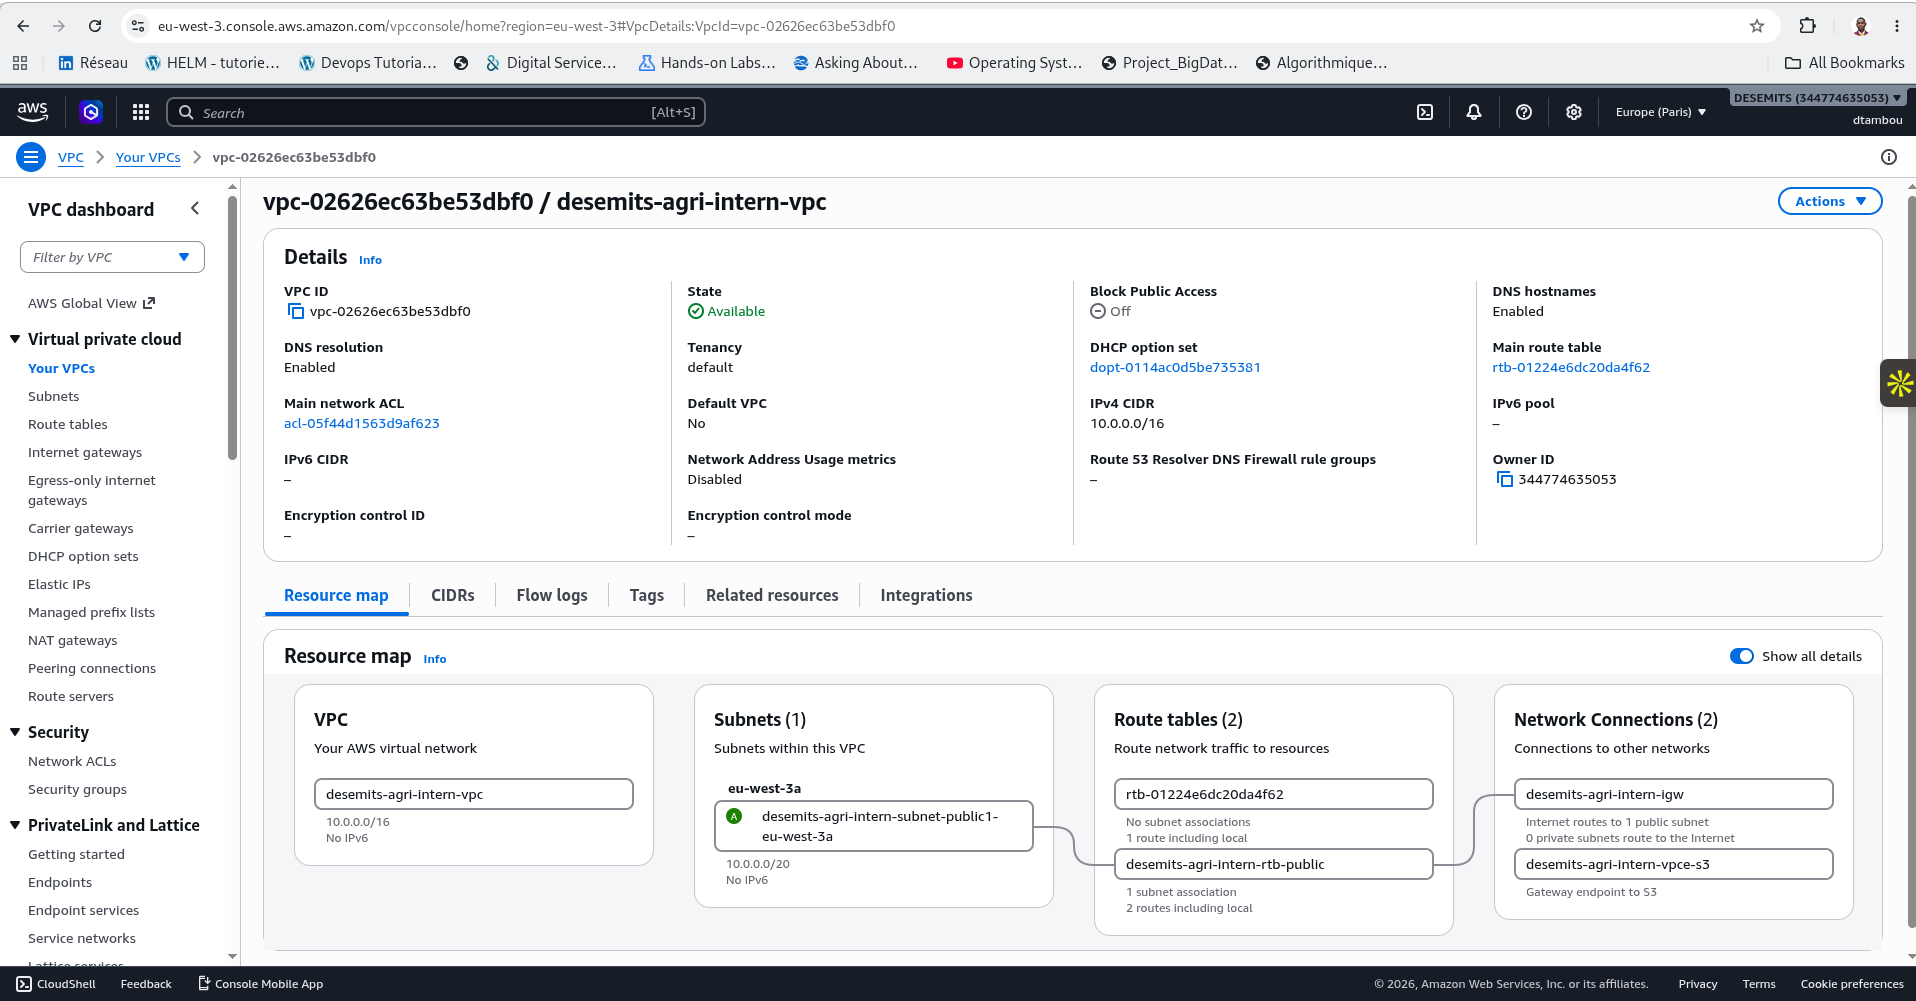
\includegraphics[width=0.85\textwidth, height=6cm, keepaspectratio]{images/vpc.png}
% \rule{0.85\textwidth}{6cm}
\caption{Virtual Private Cloud (VPC) créé pour l'isolation du projet}
\label{fig:vpc}
\end{figure}

\subsubsection{L'espace de stockage : Amazon S3 (Data Lake)}
Le composant matériel de stockage de notre architecture est un compartiment (\textit{bucket}) Amazon S3 faisant office de Data Lake. Afin d'assurer une traçabilité stricte du cycle de vie de la donnée, ce stockage a été structuré en plusieurs répertoires distincts, séparant hermétiquement les images brutes des résultats finaux et des journaux d'exécution.

\begin{table}[H]
\centering
\caption{Organisation du Data Lake sur Amazon S3}
\label{tab:datalake}
\renewcommand{\arraystretch}{1.3}
\begin{tabular}{|p{3.5cm}|p{9.8cm}|}
\hline
\textbf{Répertoire} & \textbf{Contenu et rôle} \\
\hline
\texttt{PCA/} & Contient les données transformées après réduction de dimension par Analyse en Composantes Principales (ACP). \\
\hline
\texttt{Results\_features/} & Stocke les caractéristiques extraites ainsi que les résultats intermédiaires et finaux. \\
\hline
\texttt{Test/} & Jeu de données de test utilisé pour l'évaluation et la validation du modèle. \\
\hline
\texttt{Test-grand/} & Version étendue du jeu de test pour les expérimentations à plus grande échelle. \\
\hline
\texttt{models/} & Contient les modèles entraînés ainsi que les fichiers nécessaires à leur déploiement. \\
\hline
\texttt{error-logs/} & Regroupe les journaux d'exécution générés par Amazon EMR pour assurer le débogage. \\
\hline
\texttt{studios/} & Répertoire utilisé par Amazon EMR Studio pour le stockage des espaces de travail. \\
\hline
\texttt{bootstrap-emr.sh} & Script d'initialisation exécuté lors du démarrage du cluster EMR. \\
\hline
\end{tabular}
\end{table}

\begin{figure}[H]
\centering
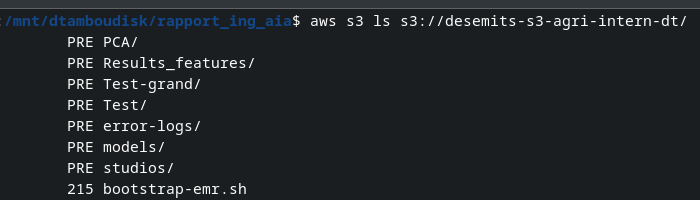
\includegraphics[width=0.95\textwidth]{images/tree.png}
% \rule{0.95\textwidth}{5cm}
\caption{Organisation du Data Lake dans le bucket Amazon S3}
\label{fig:s3bucket}
\end{figure}

\subsubsection{Le moteur de calcul : Amazon EMR}
Une fois les données sécurisées, un cluster Amazon EMR a été déployé pour exécuter les calculs. Il est composé d'un nœud maître (orchestrateur) et de plusieurs nœuds de travail (\textit{workers}) chargés de paralléliser les tâches. Une connexion sécurisée au nœud maître peut être établie via le protocole SSH pour permettre à l'administrateur d'effectuer des opérations de maintenance et d'analyse d'incidents.

\begin{figure}[H]
\centering
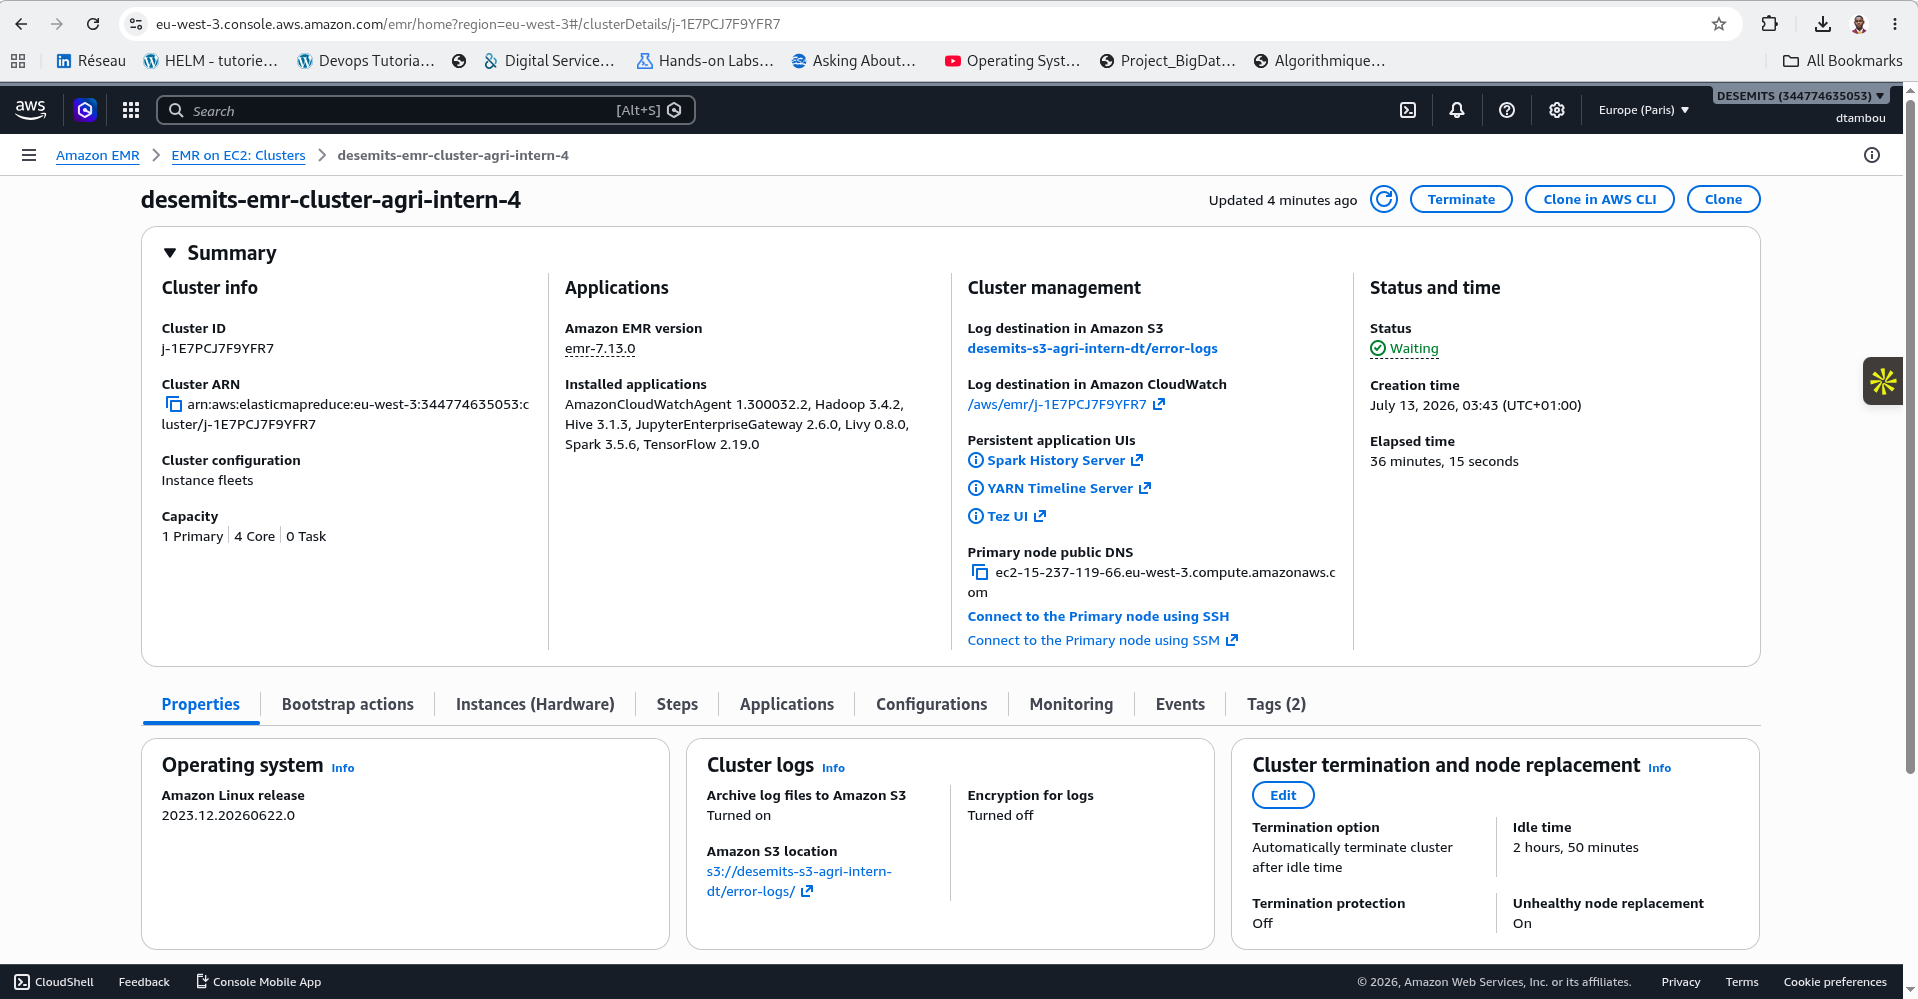
\includegraphics[width=0.95\textwidth]{images/cluster_emr1.png}
%\rule{0.95\textwidth}{5cm}
\caption{Déploiement du cluster Amazon EMR (1 Nœud maître et 4 Workers)}
\label{fig:cluster_emr}
\end{figure}

\begin{figure}[H]
\centering
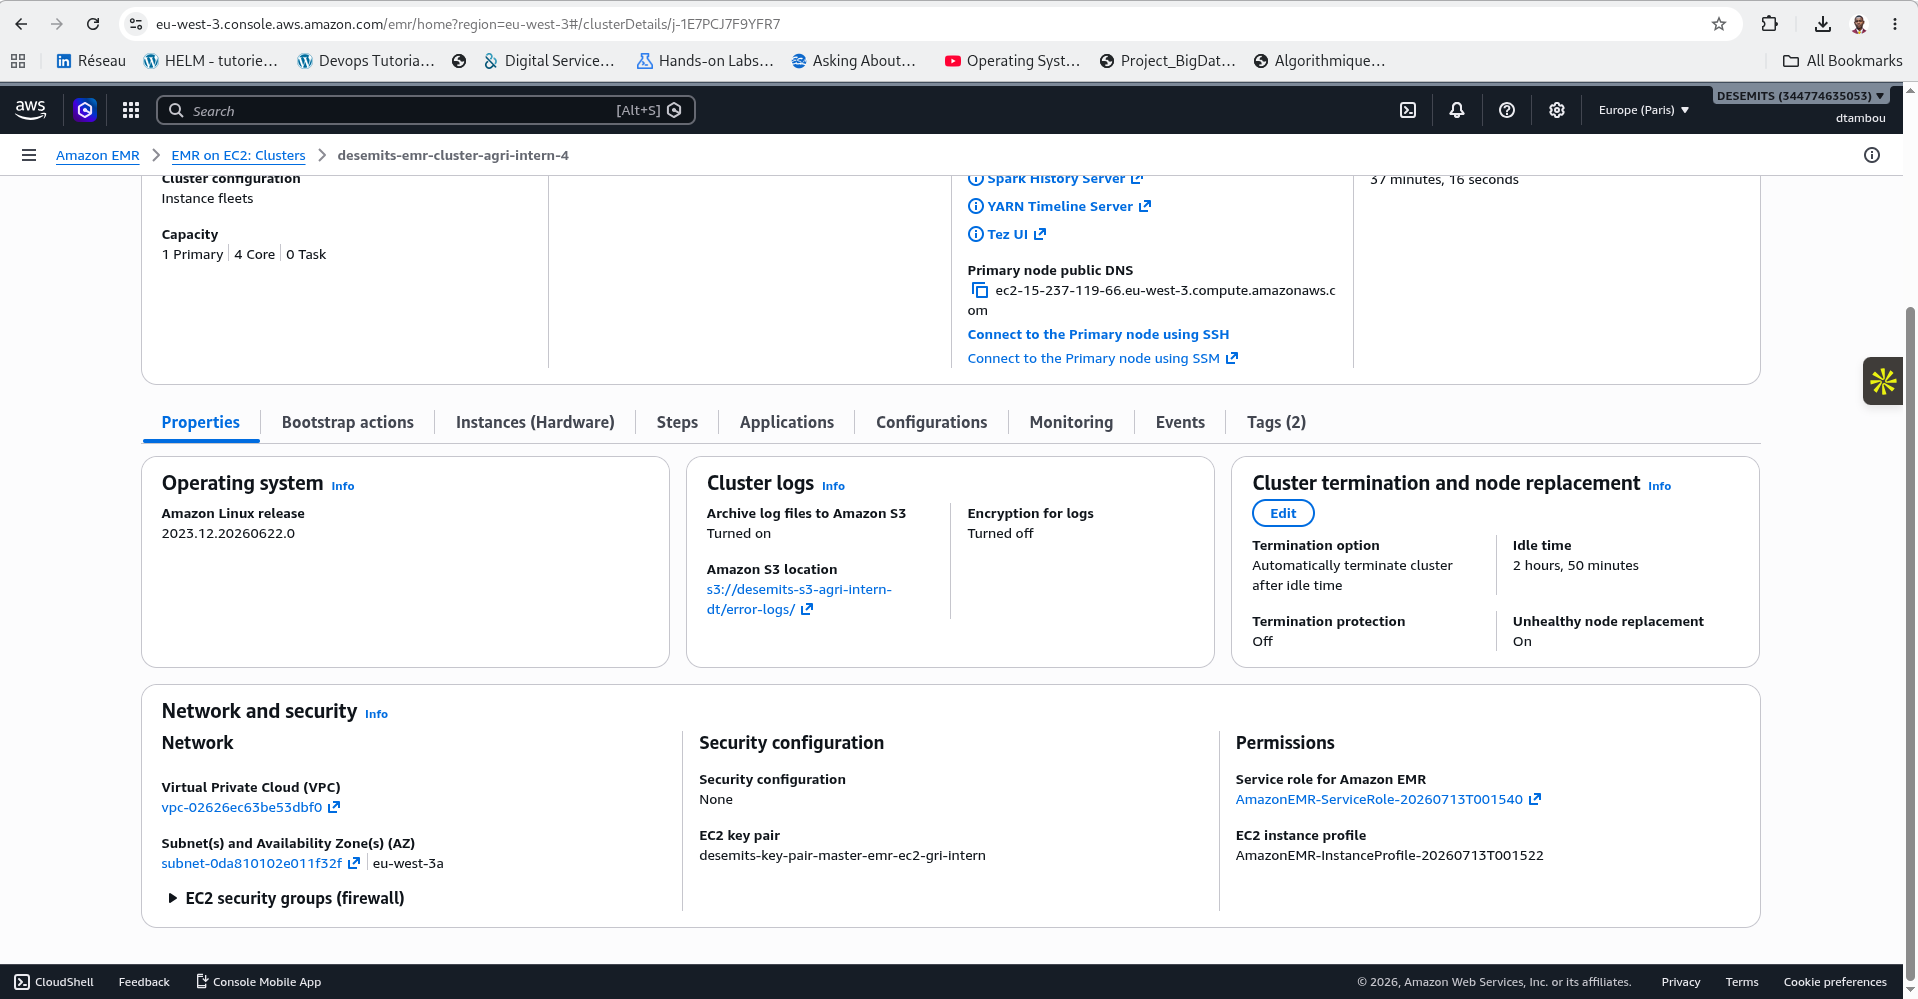
\includegraphics[width=0.95\textwidth]{images/cluster_emr2.png}
%\rule{0.95\textwidth}{5cm}
\caption{Déploiement du cluster Amazon EMR (1 Nœud maître et 4 Workers): Fin}
\label{fig:cluster_emr}
\end{figure}

\begin{figure}[H]
\centering
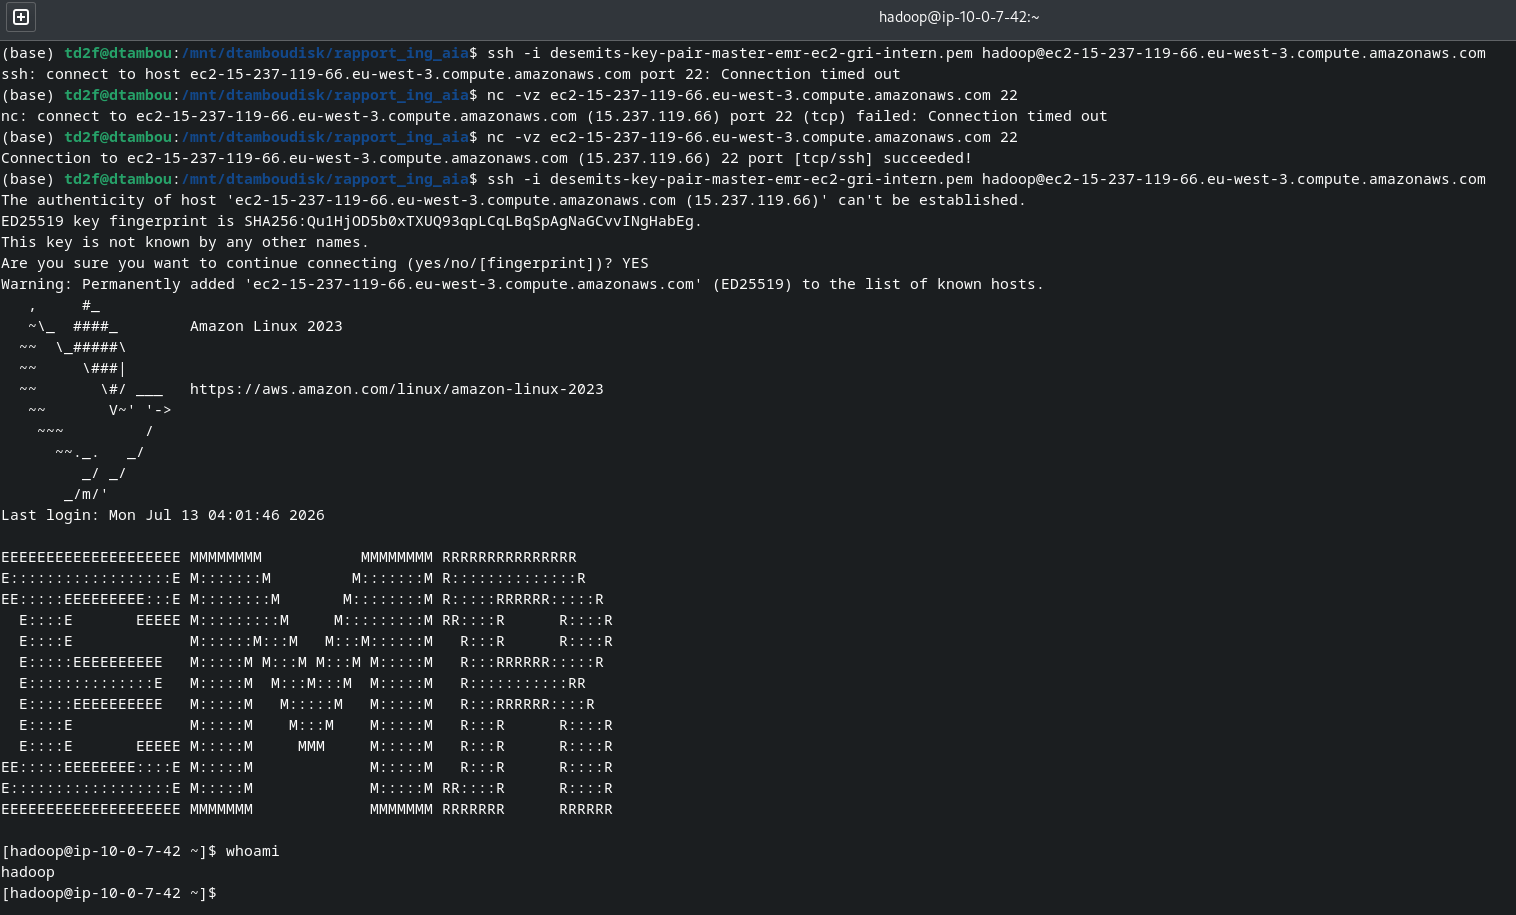
\includegraphics[width=0.85\textwidth, height=6cm, keepaspectratio]{images/connexion_ssh_master_node.png}
% \rule{0.85\textwidth}{4cm}
\caption{Connexion sécurisée au nœud maître Amazon EMR via SSH}
\label{fig:emr_ssh}
\end{figure}

\subsection{Bilan FinOps et Consommation des ressources}

\subsubsection{Consommation des ressources matérielles virtuelles}
Dans une architecture Cloud, la consommation ne se mesure pas en Watts mais en temps d'allocation de serveurs. Pour répondre à l'exigence majeure d'optimisation (FinOps), notre cluster EMR a été configuré pour être strictement \textbf{éphémère}. Il se lance au clonage d'un modèle existant et se détruit automatiquement après un temps défini (généralement 2h), évitant ainsi la consommation de ressources inactives.

\subsubsection{Calcul et optimisation des coûts}
AWS fournit des outils de suivi permettant d'analyser précisément les dépenses engendrées par chaque service utilisé. Les principaux coûts proviennent de l'exécution du cluster Amazon EMR et des instances EC2 associées. Grâce à l'extinction automatique du cluster, le budget alloué a été rigoureusement respecté pour chaque expérimentation.

% ==============================================================================
\section{Implémentation logicielle}
% ==============================================================================

L'implémentation de la partie logicielle de notre système a été réalisée en plusieurs étapes : le choix des outils, la configuration de l'environnement de travail collaboratif, et le développement des scripts de traitement distribué.

\subsection{Outils logiciels et environnement de travail collaboratif}


\subsubsection{Outils logiciels (Environnement de l'operateur metier)}
L'un des enjeux logiciels majeurs était de fournir un environnement de développement interactif, sans forcer l'utilisateur à administrer le matériel sous-jacent.

\textbf{Amazon EMR Studio :}
Il s'agit de l'interface web de développement proposée par AWS pour les traitements Big Data. Il centralise l'accès aux notebooks Jupyter et aux clusters EMR, permettant à l'utilisateur de se concentrer exclusivement sur ses données.

\begin{figure}[H]
\centering
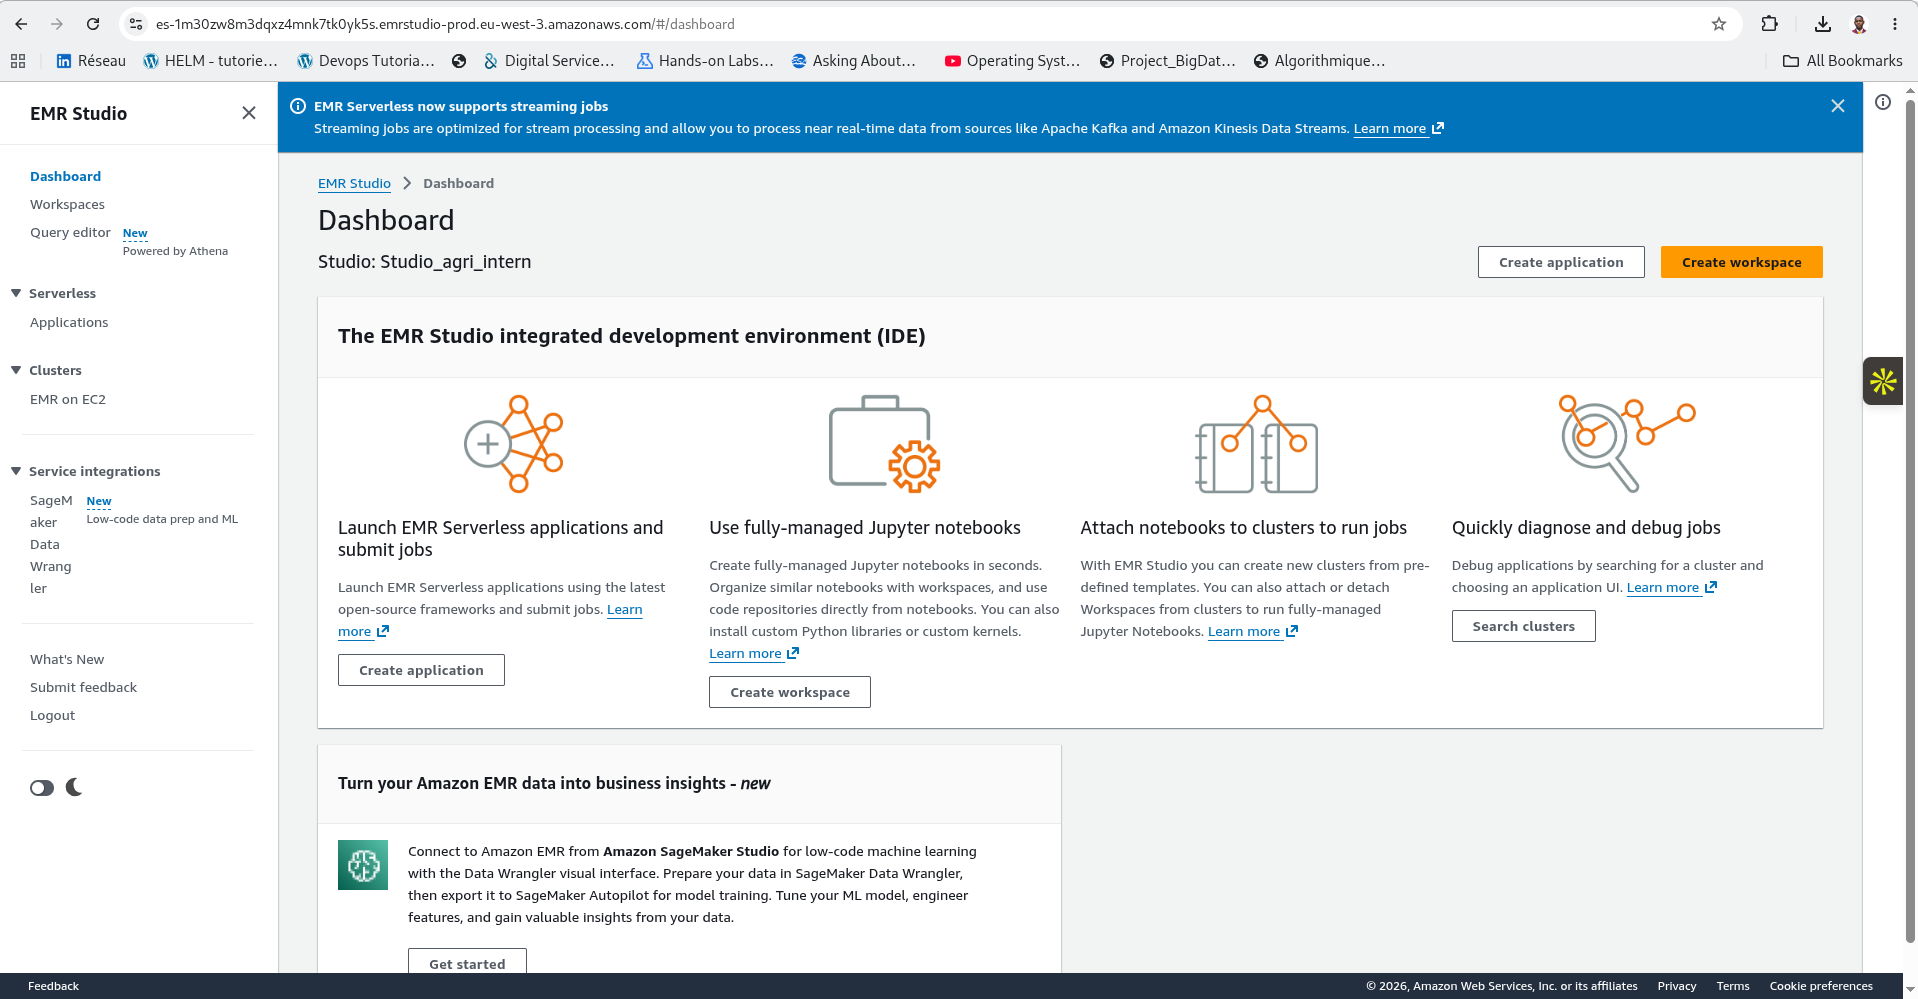
\includegraphics[width=0.95\textwidth]{images/notion_studio.png}
% \rule{0.95\textwidth}{4cm}
\caption{Interface d'Amazon EMR Studio}
\label{fig:emrstudio}
\end{figure}

\textbf{Workspace Collaboratif (Jupyter) :}
Au sein d'Amazon EMR Studio, les traitements sont réalisés dans un \textit{Workspace}. Le Workspace est totalement indépendant des ressources de calcul. Un cluster Amazon EMR peut y être attaché ou détaché selon les besoins. Cette approche permet au Data Scientist de développer ses notebooks de manière transparente, sans se préoccuper du cycle de vie du cluster éphémère.

\begin{figure}[H]
\centering
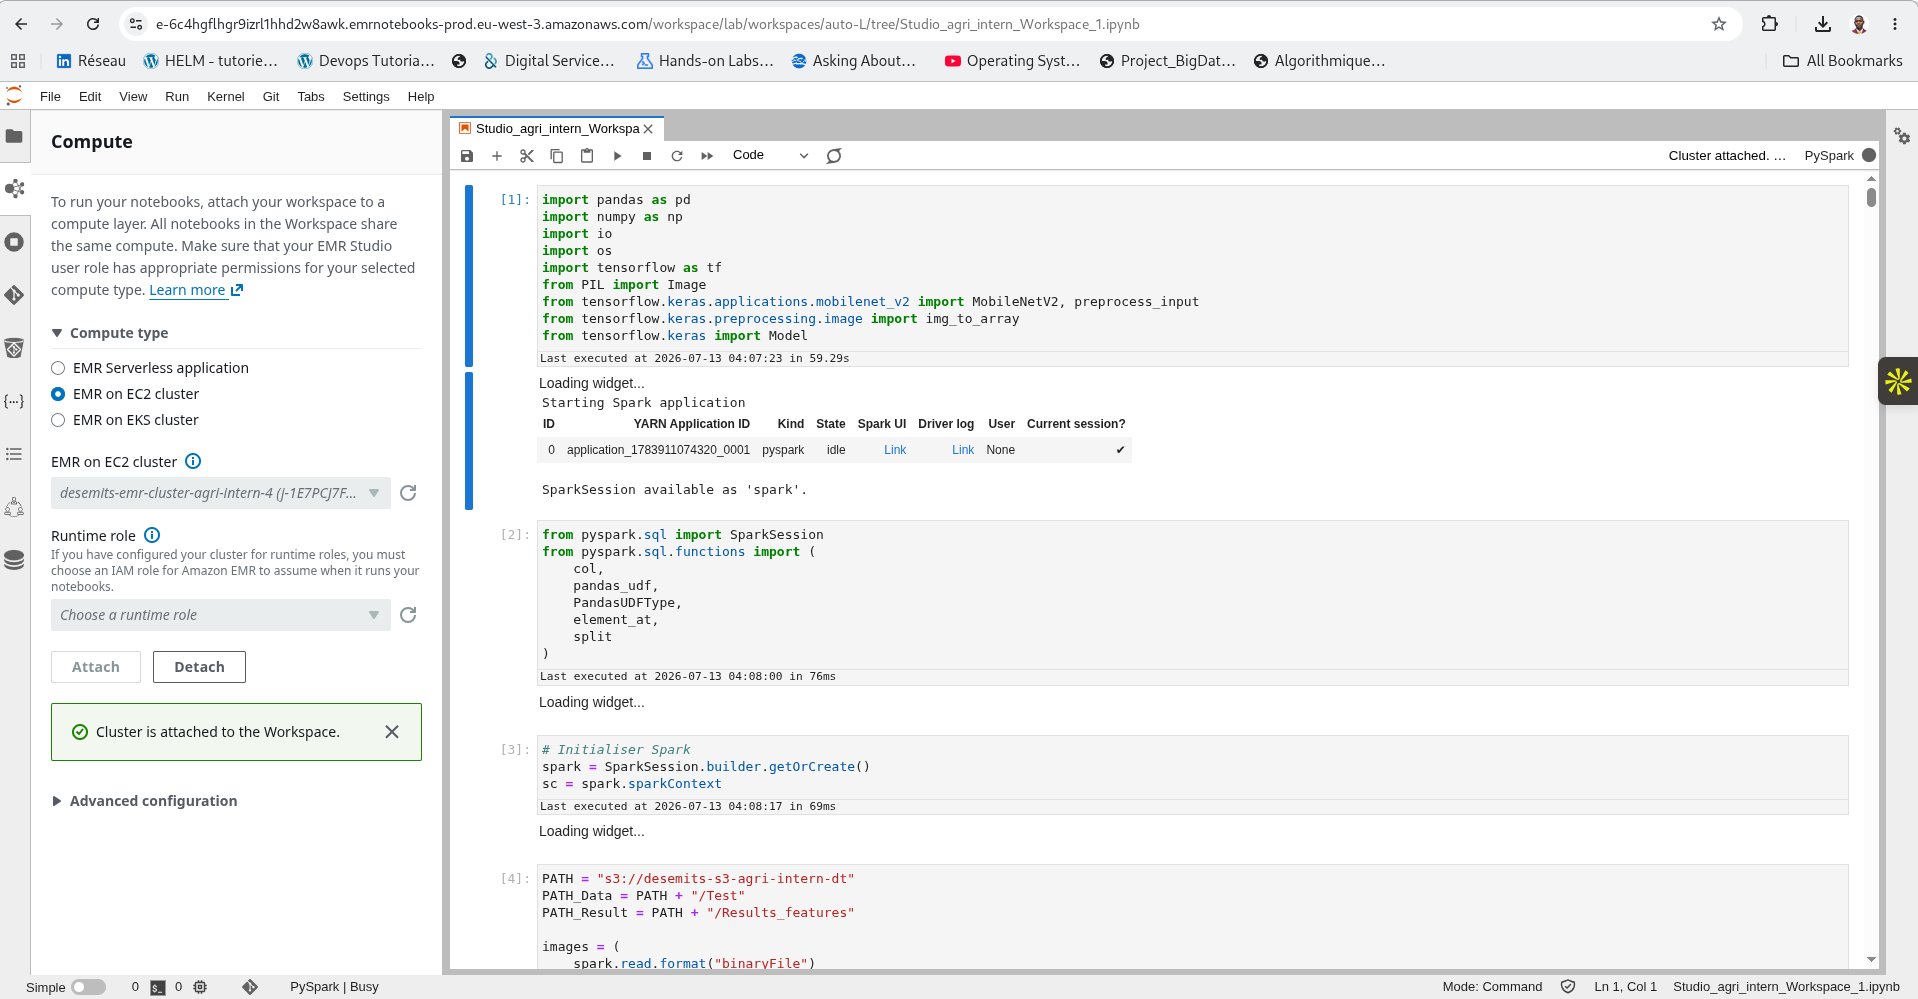
\includegraphics[width=0.95\textwidth]{images/notion_workspace_jupiter_attach_cluster.png}
% \rule{0.95\textwidth}{4cm}
\caption{Workspace collaboratif associé à un cluster Amazon EMR}
\label{fig:workspace}
\end{figure}

\subsection{Choix des technologies}

\subsubsection{Langages de programmation et Framework}
\textbf{Python :}
Langage principal utilisé pour l'ensemble des scripts de modélisation au sein de l'espace de travail. Il bénéficie d'une vaste bibliothèque facilitant la création et l'analyse de données.

\textbf{PySpark :}
Il s'agit de l'API Python pour Apache Spark, le moteur de calcul distribué. PySpark a été utilisé pour écrire le pipeline de traitement des données, distribuer l'Analyse en Composantes Principales (ACP) et paralléliser l'ingestion depuis le Data Lake S3.

\subsection{Développement des modules}
Le développement logiciel s'est concentré sur la création d'un pipeline PySpark unifié. Ce script est exécuté depuis le Workspace Jupyter et se charge de coordonner :
\begin{itemize}
    \item[$\bullet$] L'ingestion distribuée des images depuis Amazon S3.
    \item[$\bullet$] Le prétraitement et la réduction de dimensionnalité via ACP en exploitant la RAM des nœuds de travail.
    \item[$\bullet$] La sauvegarde automatisée des résultats finaux dans les sous-répertoires du Data Lake étudiés précédemment.
\end{itemize}

% ==============================================================================
\section{Résultats}
% ==============================================================================

Cette section présente les résultats obtenus lors des phases de test et de validation de notre système distribué sur AWS.

\subsection{Intégration et tests}
Les expérimentations menées ont permis de valider le bon fonctionnement de l'infrastructure Cloud distribuée. Après l'intégration du cluster EMR avec Amazon S3, les traitements ont été exécutés avec succès.

\begin{itemize}
    \item[$\bullet$] \textbf{Test de supervision via l'interface Spark :} L'interface Web native d'Apache Spark a permis de suivre en temps réel l'exécution des différents traitements. L'interface décompose chaque \textit{Job} en un ensemble de \textit{Stages}, eux-mêmes constitués de plusieurs tâches (\textit{Tasks}) exécutées en parallèle sur les différents nœuds du cluster.
\end{itemize}

\begin{figure}[H]
\centering
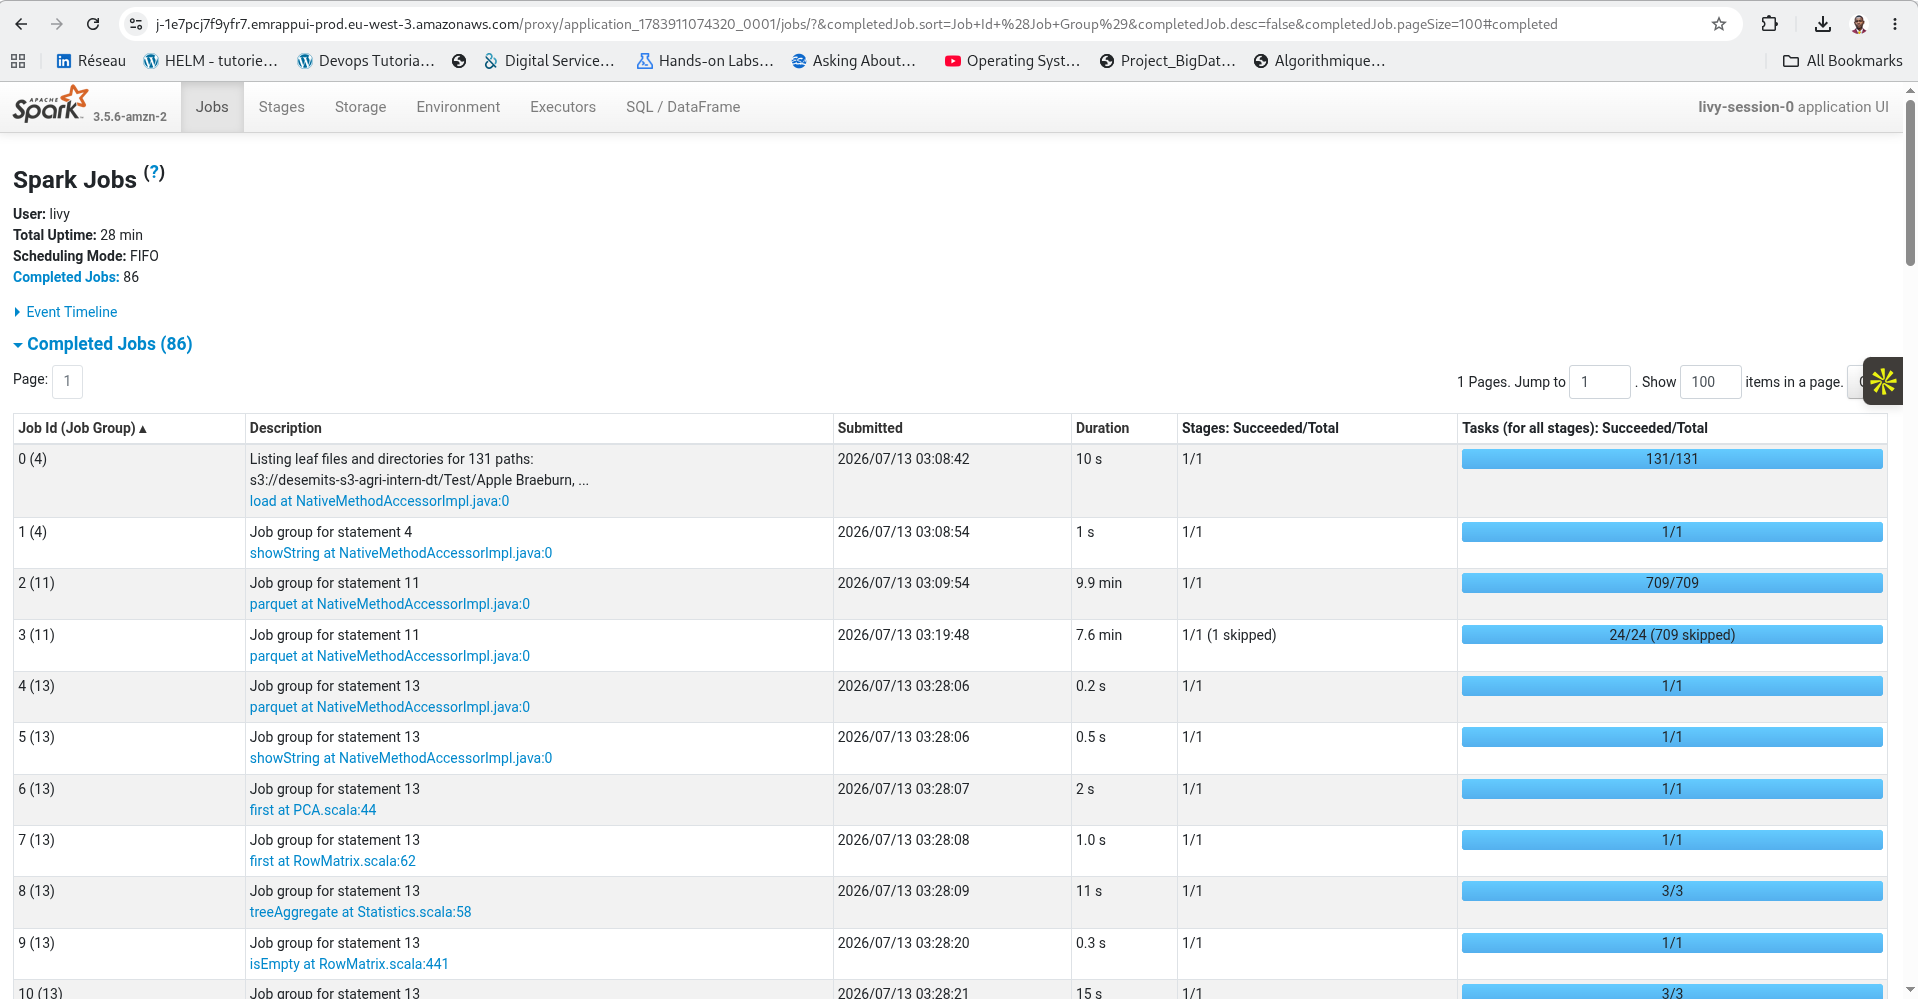
\includegraphics[width=0.95\textwidth]{images/gui_apache_spark_execution_time.png}
% \rule{0.95\textwidth}{5cm}
\caption{Interface Apache Spark présentant la répartition des tâches sur le cluster}
\label{fig:spark_jobs}
\end{figure}

\subsection{Protocole Expérimental}
Pour évaluer les performances globales du système, un protocole expérimental a été mis en place, comprenant les éléments suivants :

\subsubsection{Environnement expérimental}
Un cluster Amazon EMR instancié de manière éphémère et connecté à l'espace de travail Jupyter de l'opérateur métier. Les données sources (images) sont placées dans le répertoire S3 défini à cet effet.

\subsubsection{Scénarios de test}
Le scénario principal évalué est : « L'exécution complète du pipeline distribué PySpark sur un jeu de données volumineux, depuis le prétraitement jusqu'à l'enregistrement des résultats finaux, suivi de la libération des ressources. »

\subsubsection{Métriques de performance}
\begin{itemize}
    \item[$\bullet$] \textbf{Réussite de l'intégration :} Validation du dialogue entre le Data Lake, le Workspace et les nœuds de calcul.
    \item[$\bullet$] \textbf{Optimisation FinOps :} Validation du respect des contraintes financières par l'utilisation de clusters éphémères.
\end{itemize}

\subsection{Résultats Expérimentaux}
Le Tableau \ref{tab:evaluation} synthétise le bilan des résultats obtenus pour chaque critère.

\begin{table}[H]
\centering
\caption{Bilan de l'évaluation de l'infrastructure Cloud}
\label{tab:evaluation}
\renewcommand{\arraystretch}{1.3}
\begin{tabular}{|p{4.3cm}|p{2.2cm}|p{7cm}|}
\hline
\textbf{Critère évalué} & \textbf{Statut} & \textbf{Observation} \\
\hline
Déploiement du cluster EMR & \textbf{Validé} & Création et configuration réussies du cluster distribué Amazon EMR. \\
\hline
Stockage distribué & \textbf{Validé} & Centralisation des données et des résultats dans le Data Lake Amazon S3. \\
\hline
Exécution des traitements Spark & \textbf{Validée} & Les traitements distribués ont été exécutés et supervisés via l'interface Apache Spark sans saturation mémoire. \\
\hline
Optimisation FinOps & \textbf{Validée} & Utilisation d'un cluster éphémère limitant la consommation des ressources Cloud aux seules périodes d'exécution. \\
\hline
\end{tabular}
\end{table}

% ==============================================================================
\section{Discussion}
% ==============================================================================

Les objectifs fixés dans le cadre de ce projet ont été atteints en démontrant la faisabilité et l'efficacité d'une architecture distribuée reposant sur Amazon S3, Amazon EMR et Apache Spark. En palliant les problèmes de saturation liés à l'approche locale de l'alternant précédent, l'opérateur métier dispose désormais d'un environnement (Workspace) hautement performant.

Néanmoins, l'analyse critique des résultats révèle plusieurs pistes d'amélioration qui pourraient être envisagées pour renforcer le niveau d'automatisation de la plateforme.


% ==============================================================================
\section{Résumé du chapitre}
% ==============================================================================

Ce chapitre a présenté l'implémentation complète de l'architecture Cloud MLOps sur AWS, depuis le provisionnement de la partie matérielle virtuelle (VPC, S3, EMR) jusqu'à la mise en place de la partie logicielle (Workspaces Jupyter et PySpark). Les résultats expérimentaux confirment la faisabilité, la scalabilité et la viabilité financière de notre système pour le traitement massif d'images agricoles. La section suivante présentera la conclusion générale du mémoire et clôturera ce travail.

